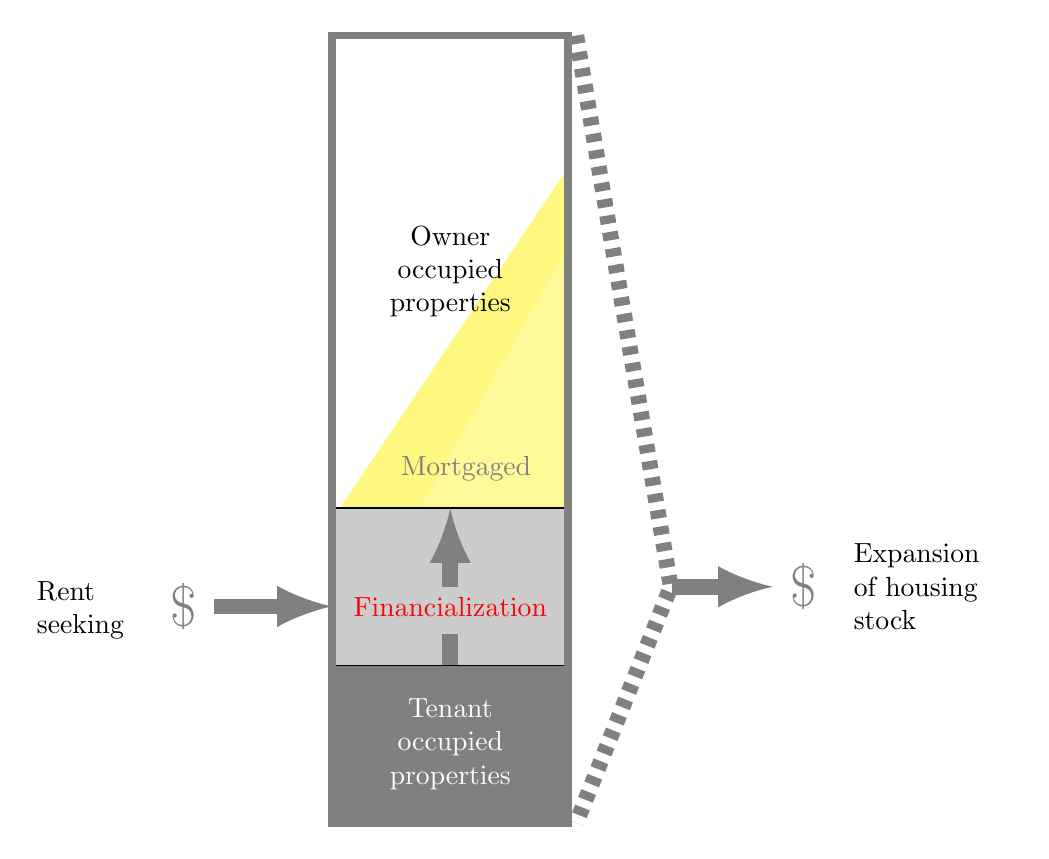
\begin{tikzpicture}{scale=.5}
\fill[yellow!50] (.1,4)--(3,4)--(3,8.33) --cycle;% MORTGAGE %Calculation. 80\%owner, so  8 above the tenant line. 2/3*8=5.333. 5.333+2=

\draw [fill=yellow!40] (0,2)--(3,2)--(3,7.33); --cycle;% MORTGAGE %Calculation. 80\%owner, so  8 above the tenant line. 2/3*8=5.333. 5.333+2=
\draw [fill=gray!40,opacity=1] (0,0) rectangle (3,4); %fiancialization   
\draw [fill=gray] (0,0) rectangle (3,2); %TENANT

\draw[line width= 1mm, black!50] (0,0) rectangle (3,10);

\node at (1.5,7)
    [text width=2.4cm, align=center]
    {\baselineskip=20pt Owner occupied properties};
\node at (1.7,4.5)
    [align=center, color=gray]
    {\baselineskip=20pt Mortgaged};
%\node at (2,3.3) [text width=2.4cm]  {\baselineskip=20pt Mortgaged};
\node at (1.5,1)
    [text width=2.4cm, align=center, white]
    {\baselineskip=20pt Tenant occupied properties};

%\draw [gray,line width=2mm](1.5,2)--(1.5,2.4) node[above, red]{Financialization}; 
\draw [gray,line width=2mm](1.5,2)--(1.5,2.4) node[above, red]{Financialization}; 
\draw [gray,-latex, line width=2mm](1.5,3)--(1.5,4);

\node at (-3,2.7)[ text width=1.5cm]{Rent seeking};
\draw [gray,line width=2mm,-latex](-1.5,2.75)node[left]{\huge$\$$}--(0,2.75);

%\node at (5.5,3)[text width=2cm]{Expansion of housing stock}; 
\draw [gray, dashed,line width=2mm,](3.1,10)--(4.3,3)--(3.1,0);

\draw [gray,line width=2mm,-latex](4.32,3)--(5.6,3)node[right]{\huge$\$$};
\node at (6.5,3)[right, text width=2cm]{Expansion of housing stock};
%\draw [gray,line width=2mm,-latex](6.5,3)--(7.5,3); 
\end{tikzpicture}


% OLDER JUST BOX LIKE ABOVE IMAGE WITHOUT FINANCIALIZATION, MONEY IN OR MONEY OUT
% \begin{figure}
% % 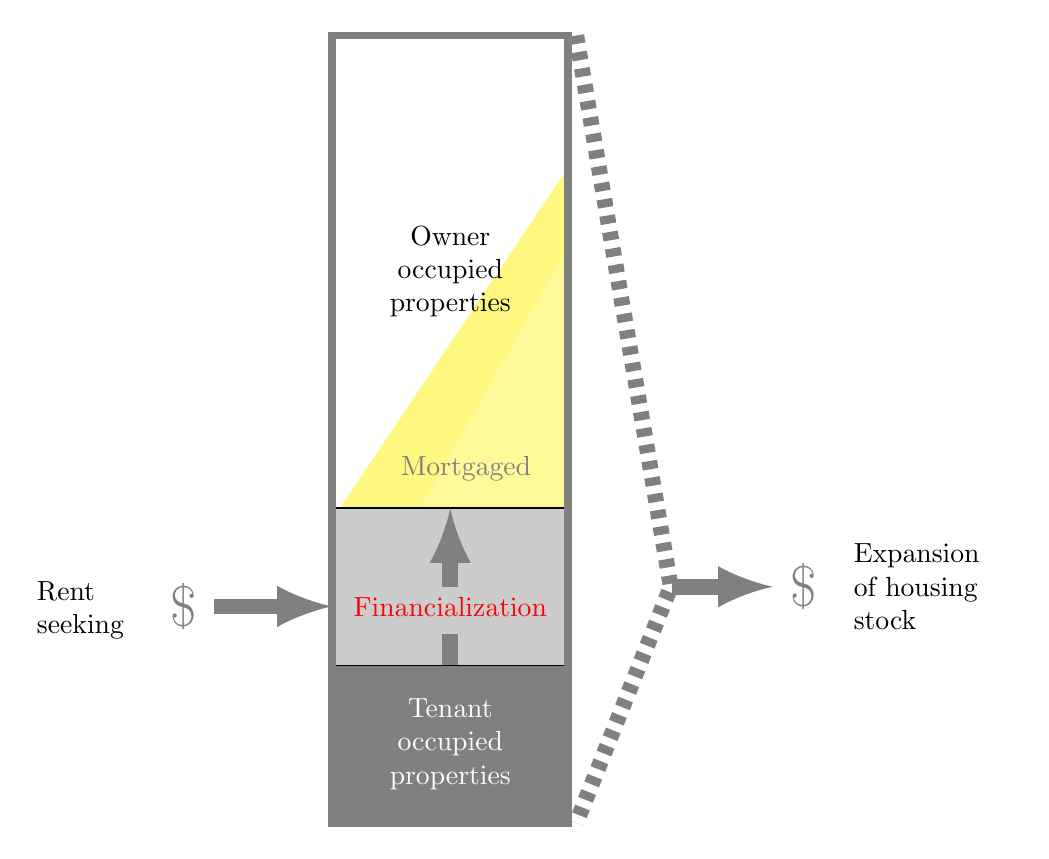
\begin{tikzpicture}{scale=.5}
\fill[yellow!50] (.1,4)--(3,4)--(3,8.33) --cycle;% MORTGAGE %Calculation. 80\%owner, so  8 above the tenant line. 2/3*8=5.333. 5.333+2=

\draw [fill=yellow!40] (0,2)--(3,2)--(3,7.33); --cycle;% MORTGAGE %Calculation. 80\%owner, so  8 above the tenant line. 2/3*8=5.333. 5.333+2=
\draw [fill=gray!40,opacity=1] (0,0) rectangle (3,4); %fiancialization   
\draw [fill=gray] (0,0) rectangle (3,2); %TENANT

\draw[line width= 1mm, black!50] (0,0) rectangle (3,10);

\node at (1.5,7)
    [text width=2.4cm, align=center]
    {\baselineskip=20pt Owner occupied properties};
\node at (1.7,4.5)
    [align=center, color=gray]
    {\baselineskip=20pt Mortgaged};
%\node at (2,3.3) [text width=2.4cm]  {\baselineskip=20pt Mortgaged};
\node at (1.5,1)
    [text width=2.4cm, align=center, white]
    {\baselineskip=20pt Tenant occupied properties};

%\draw [gray,line width=2mm](1.5,2)--(1.5,2.4) node[above, red]{Financialization}; 
\draw [gray,line width=2mm](1.5,2)--(1.5,2.4) node[above, red]{Financialization}; 
\draw [gray,-latex, line width=2mm](1.5,3)--(1.5,4);

\node at (-3,2.7)[ text width=1.5cm]{Rent seeking};
\draw [gray,line width=2mm,-latex](-1.5,2.75)node[left]{\huge$\$$}--(0,2.75);

%\node at (5.5,3)[text width=2cm]{Expansion of housing stock}; 
\draw [gray, dashed,line width=2mm,](3.1,10)--(4.3,3)--(3.1,0);

\draw [gray,line width=2mm,-latex](4.32,3)--(5.6,3)node[right]{\huge$\$$};
\node at (6.5,3)[right, text width=2cm]{Expansion of housing stock};
%\draw [gray,line width=2mm,-latex](6.5,3)--(7.5,3); 
\end{tikzpicture}


% OLDER JUST BOX LIKE ABOVE IMAGE WITHOUT FINANCIALIZATION, MONEY IN OR MONEY OUT
% \begin{figure}
% % 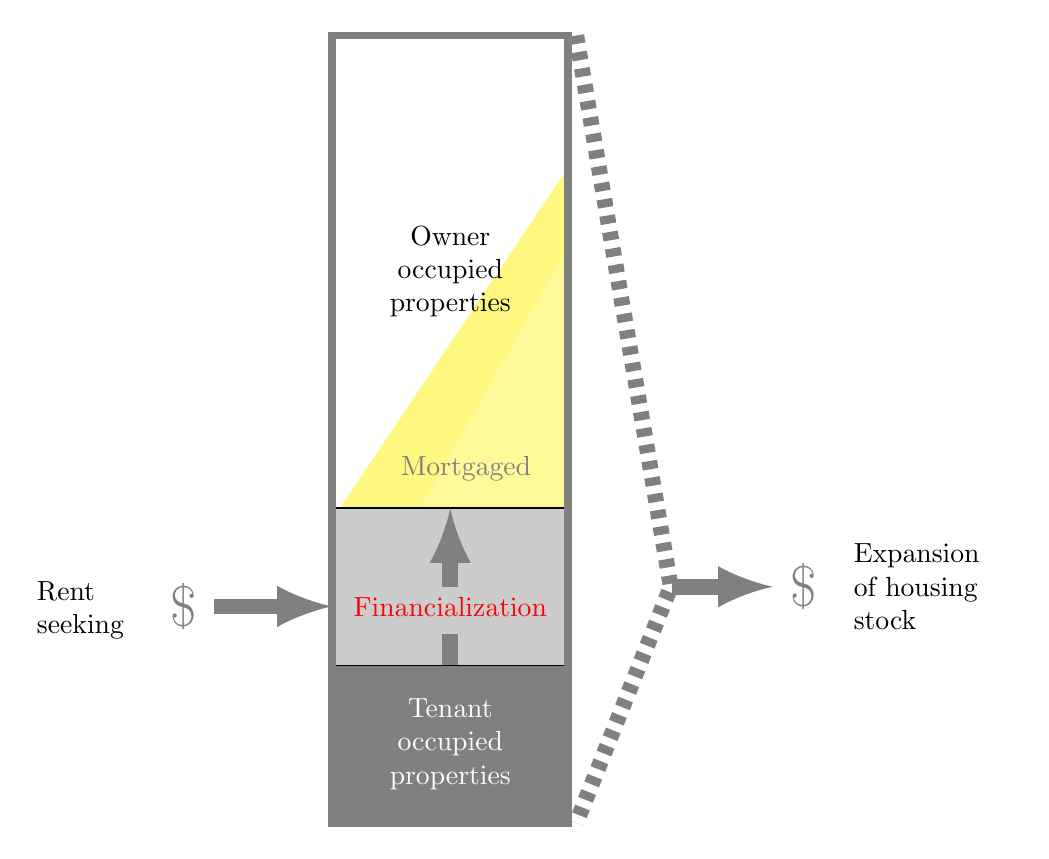
\begin{tikzpicture}{scale=.5}
\fill[yellow!50] (.1,4)--(3,4)--(3,8.33) --cycle;% MORTGAGE %Calculation. 80\%owner, so  8 above the tenant line. 2/3*8=5.333. 5.333+2=

\draw [fill=yellow!40] (0,2)--(3,2)--(3,7.33); --cycle;% MORTGAGE %Calculation. 80\%owner, so  8 above the tenant line. 2/3*8=5.333. 5.333+2=
\draw [fill=gray!40,opacity=1] (0,0) rectangle (3,4); %fiancialization   
\draw [fill=gray] (0,0) rectangle (3,2); %TENANT

\draw[line width= 1mm, black!50] (0,0) rectangle (3,10);

\node at (1.5,7)
    [text width=2.4cm, align=center]
    {\baselineskip=20pt Owner occupied properties};
\node at (1.7,4.5)
    [align=center, color=gray]
    {\baselineskip=20pt Mortgaged};
%\node at (2,3.3) [text width=2.4cm]  {\baselineskip=20pt Mortgaged};
\node at (1.5,1)
    [text width=2.4cm, align=center, white]
    {\baselineskip=20pt Tenant occupied properties};

%\draw [gray,line width=2mm](1.5,2)--(1.5,2.4) node[above, red]{Financialization}; 
\draw [gray,line width=2mm](1.5,2)--(1.5,2.4) node[above, red]{Financialization}; 
\draw [gray,-latex, line width=2mm](1.5,3)--(1.5,4);

\node at (-3,2.7)[ text width=1.5cm]{Rent seeking};
\draw [gray,line width=2mm,-latex](-1.5,2.75)node[left]{\huge$\$$}--(0,2.75);

%\node at (5.5,3)[text width=2cm]{Expansion of housing stock}; 
\draw [gray, dashed,line width=2mm,](3.1,10)--(4.3,3)--(3.1,0);

\draw [gray,line width=2mm,-latex](4.32,3)--(5.6,3)node[right]{\huge$\$$};
\node at (6.5,3)[right, text width=2cm]{Expansion of housing stock};
%\draw [gray,line width=2mm,-latex](6.5,3)--(7.5,3); 
\end{tikzpicture}


% OLDER JUST BOX LIKE ABOVE IMAGE WITHOUT FINANCIALIZATION, MONEY IN OR MONEY OUT
% \begin{figure}
% % 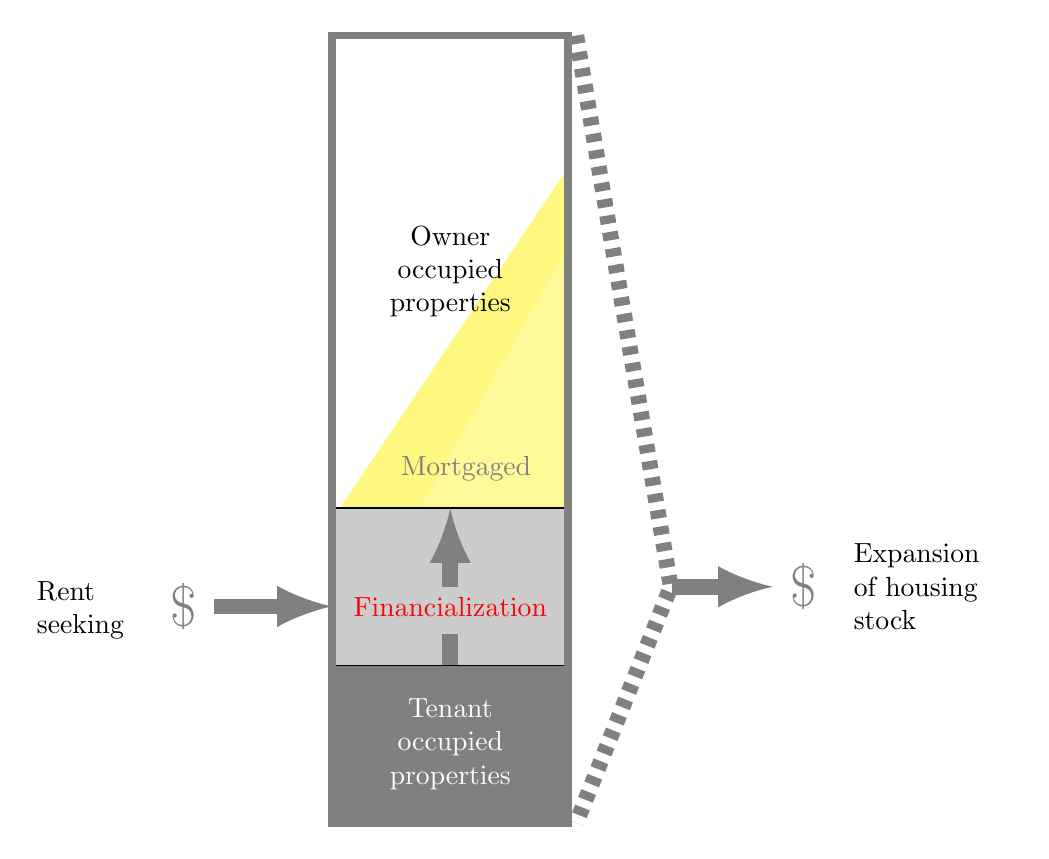
\begin{tikzpicture}{scale=.5}
\fill[yellow!50] (.1,4)--(3,4)--(3,8.33) --cycle;% MORTGAGE %Calculation. 80\%owner, so  8 above the tenant line. 2/3*8=5.333. 5.333+2=

\draw [fill=yellow!40] (0,2)--(3,2)--(3,7.33); --cycle;% MORTGAGE %Calculation. 80\%owner, so  8 above the tenant line. 2/3*8=5.333. 5.333+2=
\draw [fill=gray!40,opacity=1] (0,0) rectangle (3,4); %fiancialization   
\draw [fill=gray] (0,0) rectangle (3,2); %TENANT

\draw[line width= 1mm, black!50] (0,0) rectangle (3,10);

\node at (1.5,7)
    [text width=2.4cm, align=center]
    {\baselineskip=20pt Owner occupied properties};
\node at (1.7,4.5)
    [align=center, color=gray]
    {\baselineskip=20pt Mortgaged};
%\node at (2,3.3) [text width=2.4cm]  {\baselineskip=20pt Mortgaged};
\node at (1.5,1)
    [text width=2.4cm, align=center, white]
    {\baselineskip=20pt Tenant occupied properties};

%\draw [gray,line width=2mm](1.5,2)--(1.5,2.4) node[above, red]{Financialization}; 
\draw [gray,line width=2mm](1.5,2)--(1.5,2.4) node[above, red]{Financialization}; 
\draw [gray,-latex, line width=2mm](1.5,3)--(1.5,4);

\node at (-3,2.7)[ text width=1.5cm]{Rent seeking};
\draw [gray,line width=2mm,-latex](-1.5,2.75)node[left]{\huge$\$$}--(0,2.75);

%\node at (5.5,3)[text width=2cm]{Expansion of housing stock}; 
\draw [gray, dashed,line width=2mm,](3.1,10)--(4.3,3)--(3.1,0);

\draw [gray,line width=2mm,-latex](4.32,3)--(5.6,3)node[right]{\huge$\$$};
\node at (6.5,3)[right, text width=2cm]{Expansion of housing stock};
%\draw [gray,line width=2mm,-latex](6.5,3)--(7.5,3); 
\end{tikzpicture}


% OLDER JUST BOX LIKE ABOVE IMAGE WITHOUT FINANCIALIZATION, MONEY IN OR MONEY OUT
% \begin{figure}
% % \input{fig/financialization-expansion}
% \begin{center}
% \begin{tikzpicture}{scale=.5}
% \draw [fill=gray,] (0,0) rectangle (3,2); %TENANT
% \draw [fill=yellow!40] (0,2)--(3,2)--(3,7.33); --cycle;% MORTGAGE %Calculation. 80\%owner, so  8 above the tenant line. 2/3*8=5.333. 5.333+2=
% \draw[line width= 1mm, black!50] (0,0) rectangle (3,10);
% \node at (1.5,6)
%     [text width=2.4cm, align=center]
%     {\baselineskip=20pt\Large Owner occupied};
% \node at (2,3.3)
%     [text width=2.4cm]
%     {\baselineskip=20pt Mortgaged};
% \node at (1.5,1)
%     [text width=2.4cm, align=center, white]
%     {\baselineskip=20pt\Large Tenant occupied};
% % \caption{}
% \end{tikzpicture}
% \end{center}
% \caption{Housing tenure and mortgaged share.}
% \label{fig-mortgage-tenure}
% \end{figure}

% \begin{center}
% \begin{tikzpicture}{scale=.5}
% \draw [fill=gray,] (0,0) rectangle (3,2); %TENANT
% \draw [fill=yellow!40] (0,2)--(3,2)--(3,7.33); --cycle;% MORTGAGE %Calculation. 80\%owner, so  8 above the tenant line. 2/3*8=5.333. 5.333+2=
% \draw[line width= 1mm, black!50] (0,0) rectangle (3,10);
% \node at (1.5,6)
%     [text width=2.4cm, align=center]
%     {\baselineskip=20pt\Large Owner occupied};
% \node at (2,3.3)
%     [text width=2.4cm]
%     {\baselineskip=20pt Mortgaged};
% \node at (1.5,1)
%     [text width=2.4cm, align=center, white]
%     {\baselineskip=20pt\Large Tenant occupied};
% % \caption{}
% \end{tikzpicture}
% \end{center}
% \caption{Housing tenure and mortgaged share.}
% \label{fig-mortgage-tenure}
% \end{figure}

% \begin{center}
% \begin{tikzpicture}{scale=.5}
% \draw [fill=gray,] (0,0) rectangle (3,2); %TENANT
% \draw [fill=yellow!40] (0,2)--(3,2)--(3,7.33); --cycle;% MORTGAGE %Calculation. 80\%owner, so  8 above the tenant line. 2/3*8=5.333. 5.333+2=
% \draw[line width= 1mm, black!50] (0,0) rectangle (3,10);
% \node at (1.5,6)
%     [text width=2.4cm, align=center]
%     {\baselineskip=20pt\Large Owner occupied};
% \node at (2,3.3)
%     [text width=2.4cm]
%     {\baselineskip=20pt Mortgaged};
% \node at (1.5,1)
%     [text width=2.4cm, align=center, white]
%     {\baselineskip=20pt\Large Tenant occupied};
% % \caption{}
% \end{tikzpicture}
% \end{center}
% \caption{Housing tenure and mortgaged share.}
% \label{fig-mortgage-tenure}
% \end{figure}

% \begin{center}
% \begin{tikzpicture}{scale=.5}
% \draw [fill=gray,] (0,0) rectangle (3,2); %TENANT
% \draw [fill=yellow!40] (0,2)--(3,2)--(3,7.33); --cycle;% MORTGAGE %Calculation. 80\%owner, so  8 above the tenant line. 2/3*8=5.333. 5.333+2=
% \draw[line width= 1mm, black!50] (0,0) rectangle (3,10);
% \node at (1.5,6)
%     [text width=2.4cm, align=center]
%     {\baselineskip=20pt\Large Owner occupied};
% \node at (2,3.3)
%     [text width=2.4cm]
%     {\baselineskip=20pt Mortgaged};
% \node at (1.5,1)
%     [text width=2.4cm, align=center, white]
%     {\baselineskip=20pt\Large Tenant occupied};
% % \caption{}
% \end{tikzpicture}
% \end{center}
% \caption{Housing tenure and mortgaged share.}
% \label{fig-mortgage-tenure}
% \end{figure}
